\documentclass[10pt]{beamer}

\usetheme[progressbar=frametitle]{metropolis}

\usepackage[absolute,overlay]{textpos}
\usepackage{booktabs}
\usepackage[scale=2]{ccicons}
%\usepackage[brazilian]{babel}
%\usepackage[T1]{fontenc}    % Selecao de codigos de fonte.
\usepackage[utf8]{inputenc} 

\usepackage{pgfplots}
\usepgfplotslibrary{dateplot}

\usepackage{xspace}
\newcommand{\themename}{\textbf{\textsc{metropolis}}\xspace}

\title{Aplicando a Teoria Mie-Debye para Caracterização de Parâmetros Físicos \\em Pinças Óticas}
\subtitle{Defesa de Dissertação de Mestrado}
\date{\today}
\author{Arthur Luna da Fonseca}
\date{\today}
\institute{Instituto de Física - Universidade Federal do Rio de Janeiro}
\titlegraphic{\hfill
\includegraphics[height=2.cm]{../logo_ufrj}}

\begin{document}

\maketitle

%%%%%%%%%%%%%%%%%%%%%%%%%%%%%%%%%%%%%%%%%%%%%%%%%%%%%%%%%%%%%%%%%%%%%%%%%%%%%%%%%%%%%%%%%%%%%%%%%

\begin{frame}{Conteúdo}
  \setbeamertemplate{section in toc}[sections numbered]
  \tableofcontents[hideallsubsections]
\end{frame}

%%%%%%%%%%%%%%%%%%%%%%%%%%%%%%%%%%%%%%%%%%%%%%%%%%%%%%%%%%%%%%%%%%%%%%%%%%%%%%%%%%%%%%%%%%%%%%%%%

\section{Introdução}

%%%%%%%%%%%%%%%%%%%%%%%%%%%%%%%%%%%%%%%%%%%%%%%%%%%%%%%%%%%%%%%%%%%%%%%%%%%%%%%%%%%%%%%%%%%%%%%%%

\begin{frame}[fragile]{Introdução}
      \begin{center}
          \metroset{block=fill}
          \begin{exampleblock}{Goal}
            Describe the process of scattering of EM waves by a spherically symmetric object.\\
            Discuss the application of this model to experiments that try to measure Casimir interactions.
          \end{exampleblock}
      \end{center}
\end{frame}

%%%%%%%%%%%%%%%%%%%%%%%%%%%%%%%%%%%%%%%%%%%%%%%%%%%%%%%%%%%%%%%%%%%%%%%%%%%%%%%%%%%%%%%%%%%%%%%%%

\begin{frame}[fragile]{Introduction}

Path: \\
    \begin{center}
        Find a solution for a scalar wave equation in spherical coordinates 

        $\downarrow$

        Adapt the result to a vector field $\rightarrow$ Electromagnetic field description

        $\downarrow$

        Scattering description with developed tools

        $\downarrow$

        Aplications

    \end{center}

\end{frame}

%%%%%%%%%%%%%%%%%%%%%%%%%%%%%%%%%%%%%%%%%%%%%%%%%%%%%%%%%%%%%%%%%%%%%%%%%%%%%%%%%%%%%%%%%%%%%%%%%

\section{Spherical Wave Solutions of the Scalar Wave Equation}

%%%%%%%%%%%%%%%%%%%%%%%%%%%%%%%%%%%%%%%%%%%%%%%%%%%%%%%%%%%%%%%%%%%%%%%%%%%%%%%%%%%%%%%%%%%%%%%%%

\begin{frame}[fragile]{Spherical Wave Solutions of the Scalar Wave Equation}
    Consider the scalar function $\psi(\vec{r},\omega)$, which satisfies the Helmholtz wave equation\\
      \begin{equation*}
        \left(\nabla^2 + k^2\right)\psi(\vec{r},\omega) = 0 .
      \end{equation*}

    Note that $k^2=\omega^2/c^2$ and $\psi(\vec{r},\omega)=FT_t{\psi(\vec{r},t)}$.

\end{frame}

%%%%%%%%%%%%%%%%%%%%%%%%%%%%%%%%%%%%%%%%%%%%%%%%%%%%%%%%%%%%%%%%%%%%%%%%%%%%%%%%%%%%%%%%%%%%%%%%%

\begin{frame}[fragile]{Spherical Wave Solutions of the Scalar Wave Equation}

The laplacian $\nabla$ is then writen in spherical coordinates and, after separating the variables and solving the angular part, we find:
  \begin{equation*}
    \psi(\vec{r},\omega)=\sum_{l,m}F_{l,m}(r)Y_{l,m}(\theta,\phi)
  \end{equation*}
and $F_{l,m}(r)$ is the solution for the radial part of the equation (don't depend on m).

With the transformation:
  \begin{equation*}
      F_l(r)=\frac{1}{\sqrt[]{r}}u_l(r)
  \end{equation*}
the radial part of the equation becomes a Bessel equation, which solutions are:
\begin{equation*}
F_l(r)=\frac{1}{\sqrt[]{r}}\left( A_{l,m}J_{l+1/2}(r) + B_{l,m}N_{l+1/2}(r) \right)
\end{equation*}

\end{frame}

%%%%%%%%%%%%%%%%%%%%%%%%%%%%%%%%%%%%%%%%%%%%%%%%%%%%%%%%%%%%%%%%%%%%%%%%%%%%%%%%%%%%%%%%%%%%%%%%%

\begin{frame}[fragile]{Spherical Wave Solutions of the Scalar Wave Equation}

Now, we define the \emph{Spherical Bessel and Henkel Functions}:
  \begin{equation*}
    \begin{split}
      j_l(kr)=\left(\frac{\pi}{2kr}\right)^{1/2}J_{l+1/2}(kr)\\
      n_l(kr)=\left(\frac{\pi}{2kr}\right)^{1/2}N_{l+1/2}(kr)\\
      h_l^{\pm}(kr)=j_l(kr)\pm i n_l(kr)\\
    \end{split}
  \end{equation*}
which look like:
        \begin{textblock*}{3cm}(2.2cm,7cm)
        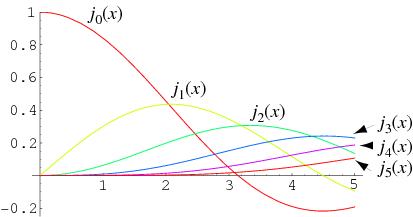
\includegraphics[width=4cm]{besselesf1}
        \end{textblock*}
        \begin{textblock*}{3cm}(7.2cm,6.5cm)
        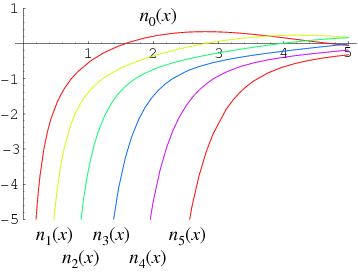
\includegraphics[width=4cm]{besselesf2}
        \end{textblock*}

\end{frame}

%%%%%%%%%%%%%%%%%%%%%%%%%%%%%%%%%%%%%%%%%%%%%%%%%%%%%%%%%%%%%%%%%%%%%%%%%%%%%%%%%%%%%%%%%%%%%%%%%

\begin{frame}[fragile]{Spherical Wave Solutions of the Scalar Wave Equation}
    When $kr>>l$, those functions will behave as follows:
      \begin{equation*}
        \begin{split}
          j_l(kr)\rightarrow \frac{1}{kr}sin\left(kr-\frac{l\pi}{2}\right)\\
          n_l(kr)\rightarrow -\frac{1}{kr}cos\left(kr-\frac{l\pi}{2}\right)\\
          h_l^{+}(kr)\rightarrow (-i)^{l+1} \frac{e^{ikr}}{kr}\\
        \end{split}
      \end{equation*}
Now, we have a complete set of functions to describe $\psi$:
      \begin{equation*}
          \psi({\bf r},\omega)=\sum_{l,m} [A^{(+)}_{lm}h^{(+)}_l(kr) + A^{(-)}_{lm}h^{(-)}_l(kr)]Y_{lm}(\theta,\phi)
      \end{equation*}

\end{frame}

%%%%%%%%%%%%%%%%%%%%%%%%%%%%%%%%%%%%%%%%%%%%%%%%%%%%%%%%%%%%%%%%%%%%%%%%%%%%%%%%%%%%%%%%%%%%%%%%%

\section{Electromagnetic Fields description}

%%%%%%%%%%%%%%%%%%%%%%%%%%%%%%%%%%%%%%%%%%%%%%%%%%%%%%%%%%%%%%%%%%%%%%%%%%%%%%%%%%%%%%%%%%%%%%%%%

\begin{frame}[fragile]{Electromagnetic Fields description}

Motivation: 
  \begin{center}
  Right now we have the wave equation solution for a scalar field.

  Transverse field can be obtained by multiplying the solution by a transverse vector.

  \alert{But which transverse vector?}
  \end{center}
        \begin{textblock*}{3cm}(4.8cm,6.5cm)
            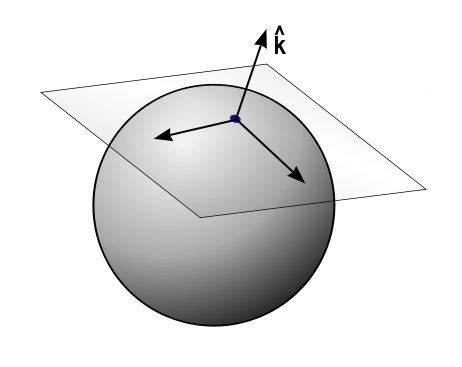
\includegraphics[width=3.6cm]{tangesfk}
        \end{textblock*}

\end{frame}

%%%%%%%%%%%%%%%%%%%%%%%%%%%%%%%%%%%%%%%%%%%%%%%%%%%%%%%%%%%%%%%%%%%%%%%%%%%%%%%%%%%%%%%%%%%%%%%%%

\begin{frame}[fragile]{Electromagnetic Fields description}

The vector operator $\nabla_k$ (in reciprocal space) is a good way to start. Assuming the field has no longitudinal component ($\vec{k} \cdot \vec{A}=0$), we can write the operator as:
      \begin{equation*}
          \nabla_k = \frac{1}{k}\left(\hat{\theta}\frac{\partial}{\partial\theta} + \hat{\phi}\frac{1}{sen\theta}\frac{\partial}{\partial\phi}\right)
      \end{equation*}
where is clear that it is defined in the tangencial plane.
        \begin{textblock*}{3cm}(4.8cm,6.5cm)
            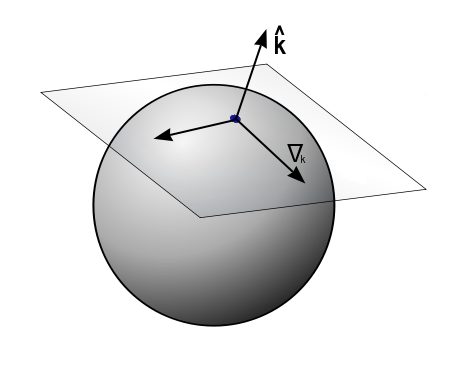
\includegraphics[width=3.6cm]{tangesfkd}
        \end{textblock*}
\end{frame}

%%%%%%%%%%%%%%%%%%%%%%%%%%%%%%%%%%%%%%%%%%%%%%%%%%%%%%%%%%%%%%%%%%%%%%%%%%%%%%%%%%%%%%%%%%%%%%%%%

\begin{frame}[fragile]{Electromagnetic Fields description}

Now, the last component should be perpendicular to, not just $\hat{k}$, but also $\nabla_k$. The obvious choice is to take the vector product:
      \begin{equation*}
          \hat{k}\times\nabla_k = \alpha \vec{L}
      \end{equation*}
and, now, we finally have a set of vetors that describes our vector field:
        \begin{textblock*}{3cm}(4.8cm,6.5cm)
            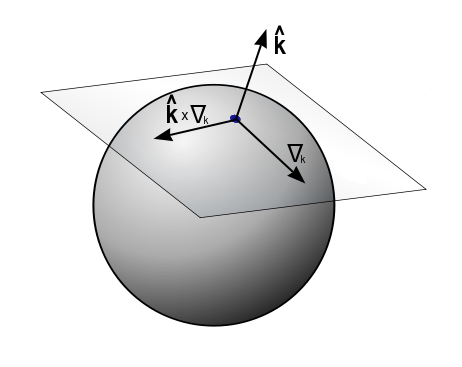
\includegraphics[width=3.6cm]{tangesfkdk}
        \end{textblock*}

\end{frame}

%%%%%%%%%%%%%%%%%%%%%%%%%%%%%%%%%%%%%%%%%%%%%%%%%%%%%%%%%%%%%%%%%%%%%%%%%%%%%%%%%%%%%%%%%%%%%%%%%

\begin{frame}[fragile]{Electromagnetic Fields description}

Since the spherical harmonics are eigenfunctions of the operator $\vec{L}$, we can build our fields with the normalized vector
      \begin{equation*}
          \vec{X}_{lm}(\theta,\phi)=\frac{1}{\sqrt[]{l(l+1)}}\vec{L}Y_{lm}(\theta,\phi).
      \end{equation*}
First, we build the magnetic multipole field, using the scalar field expansion found earlier:
      \begin{equation*}
      \begin{split}
          \vec{E}_{lm}^{(M)}(\vec{r})=c^2g_l(kr)\vec{X}_{lm}(\theta,\phi)\\
          \vec{B}_{lm}^{(M)}(\vec{r})=\frac{-i}{kc^2}\nabla \times \vec{E}_{lm}^{(M)}(\vec{r})
      \end{split}
      \end{equation*}
where
      \begin{equation*}
          g_l(kr)= B^{(+)}_{l}h^{(+)}_l(kr) + B^{(-)}_{l}h^{(-)}_l(kr).
      \end{equation*}
\end{frame}

%%%%%%%%%%%%%%%%%%%%%%%%%%%%%%%%%%%%%%%%%%%%%%%%%%%%%%%%%%%%%%%%%%%%%%%%%%%%%%%%%%%%%%%%%%%%%%%%%

\begin{frame}[fragile]{Electromagnetic Fields description}
The same ideia is used to construct the eletric multipole field, which leads us to the final result:
      \begin{equation*}
      \begin{split}
          \vec{E}(\vec{r})=c^2\sum_{l,m}\left[ \frac{i}{k}a_E(l,m)\nabla \times f_l(kr)\vec{X}_{lm}(\theta,\phi) + a_M(l,m)g_l(kr)\vec{X}_{lm}(\theta,\phi)  \right],\\
          \vec{B}(\vec{r})=\sum_{l,m}\left[ a_E(l,m)f_l(kr)\vec{X}_{lm}(\theta,\phi) - \frac{-i}{k} a_M(l,m)\nabla \times g_l(kr)\vec{X}_{lm}(\theta,\phi)) \right].
      \end{split}
      \end{equation*}

\end{frame}

%%%%%%%%%%%%%%%%%%%%%%%%%%%%%%%%%%%%%%%%%%%%%%%%%%%%%%%%%%%%%%%%%%%%%%%%%%%%%%%%%%%%%%%%%%%%%%%%%

\begin{frame}[fragile]{Electromagnetic Fields description}

Plane waves also have a spherical wave expansion. As an example, we have the case of $\hat{k}=\hat{z}$:
      \begin{equation*}
          e^{ikz}= \sum_{l=0}^{\infty}i^l(2l+1)j_l(kr)P_l(cos\theta))
      \end{equation*}
      where
      \begin{equation*}
          P_l(cos\theta)=Y_{l0}(\theta)
      \end{equation*}


\end{frame}

%%%%%%%%%%%%%%%%%%%%%%%%%%%%%%%%%%%%%%%%%%%%%%%%%%%%%%%%%%%%%%%%%%%%%%%%%%%%%%%%%%%%%%%%%%%%%%%%%

\begin{frame}[fragile]{Electromagnetic Fields description}

This leads to the field:
      \begin{equation*}
      \begin{split}
          \vec{E}(\vec{r})=\sum_{l=1}^{\infty}i^l\sqrt[]{4\pi(2l+1)}\left[j_l(kr)\vec{X}_{l,\pm1}(\theta,\phi) \pm \frac{1}{k}\nabla \times j_l(kr)\vec{X}_{l,\pm1}(\theta,\phi)  \right],\\
          \vec{B}(\vec{r})=\frac{1}{c}\sum_{l=1}^{\infty}i^l\sqrt[]{4\pi(2l+1)}\left[ \frac{-i}{k}\nabla \times j_l(kr)\vec{X}_{l,\pm1}(\theta,\phi) \mp  ij_l(kr)\vec{X}_{l,\pm1}(\theta,\phi)\right].
      \end{split}
      \end{equation*}
Those will be a sum of \emph{ingoing} spherical waves of various $l$'s.
\end{frame}

%%%%%%%%%%%%%%%%%%%%%%%%%%%%%%%%%%%%%%%%%%%%%%%%%%%%%%%%%%%%%%%%%%%%%%%%%%%%%%%%%%%%%%%%%%%%%%%%%

\section{Scattering of Electromagnetic Waves by a sphere (Mie)}

%%%%%%%%%%%%%%%%%%%%%%%%%%%%%%%%%%%%%%%%%%%%%%%%%%%%%%%%%%%%%%%%%%%%%%%%%%%%%%%%%%%%%%%%%%%%%%%%%

\begin{frame}[fragile]{Scattering of Electromagnetic Waves by a sphere (Mie)}
We begin to discuss our problem by stating that we can divide our fields in 2 parts:
      \begin{equation*}
      \begin{split}
          \vec{E}(\vec{r}) = \vec{E}_{inc}(\vec{r}) + \vec{E}_{sc}(\vec{r})\\
          \vec{B}(\vec{r}) = \vec{B}_{inc}(\vec{r}) + \vec{B}_{sc}(\vec{r})
      \end{split}
      \end{equation*}

      We use the multipole basis to describe them all! But with caution...

\end{frame}

%%%%%%%%%%%%%%%%%%%%%%%%%%%%%%%%%%%%%%%%%%%%%%%%%%%%%%%%%%%%%%%%%%%%%%%%%%%%%%%%%%%%%%%%%%%%%%%%%

\begin{frame}[fragile]{Scattering of Electromagnetic Waves by a sphere (Mie)}
$\vec{A}_{inc}(\vec{r})$ is an incoming wave, described by the plane wave expansion.

$\vec{A}_{sc}(\vec{r})$ is the scattered wave. Only one Henkel function describe \emph{outgoing} spherical wave: $H_l^+(kr)$.

      \begin{equation*}
      \begin{split}
          \vec{E}_{sc}(\vec{r})=\frac{1}{2}\sum_{l=1}^{\infty}i^l\sqrt[]{4\pi(2l+1)}\left[\alpha _{\pm}h^+_l\vec{X}_{l,\pm1} \pm \beta_{\pm}\frac{1}{k}\nabla \times h^+_l\vec{X}_{l,\pm1}\right],\\
          \vec{B}_{sc}(\vec{r})=\frac{1}{2c}\sum_{l=1}^{\infty}i^l\sqrt[]{4\pi(2l+1)}\left[\alpha_{\pm}\frac{-i}{k}\nabla \times h^+_l\vec{X}_{l,\pm1} \mp i\beta_{\pm}h^+_l\vec{X}_{l,\pm1}\right].     
          \end{split}
      \end{equation*}

\end{frame}

%%%%%%%%%%%%%%%%%%%%%%%%%%%%%%%%%%%%%%%%%%%%%%%%%%%%%%%%%%%%%%%%%%%%%%%%%%%%%%%%%%%%%%%%%%%%%%%%%

\begin{frame}[fragile]{Scattering of Electromagnetic Waves by a sphere (Mie)}

$\alpha _{\pm}$ and $\beta_{\pm}$ are both determined by the boundary conditions.
Since the scatterer is spherically symmetric, no direction will be treated differently; and assuming there is no absorption, the scattering effect only changes the 

\end{frame}

%%%%%%%%%%%%%%%%%%%%%%%%%%%%%%%%%%%%%%%%%%%%%%%%%%%%%%%%%%%%%%%%%%%%%%%%%%%%%%%%%%%%%%%%%%%%%%%%%

\begin{frame}[fragile]{Scattering of Electromagnetic Waves by a sphere (Mie)}


\end{frame}

%%%%%%%%%%%%%%%%%%%%%%%%%%%%%%%%%%%%%%%%%%%%%%%%%%%%%%%%%%%%%%%%%%%%%%%%%%%%%%%%%%%%%%%%%%%%%%%%%



%\begin{frame}{Animation}
%  \begin{itemize}[<+- | alert@+>]
%    \item \alert<4>{This is\only<4>{ really} important}
%    \item Now this
%    \item And now this
%  \end{itemize}
%\end{frame}



%{%
%\setbeamertemplate{frame footer}{---->Put footer in HERE}
%\begin{frame}[fragile]{Frame footer}
%    \themename defines a custom beamer template to add a text to the footer. It can be set via
%    \begin{verbatim}\setbeamertemplate{frame footer}{My custom footer}\end{verbatim}
%\end{frame}
%}

\section{Conclusion}

%\begin{frame}[standout]
%  Questions?
%\end{frame}

\appendix


\end{document}
